%!TEX root = ../dissertation.tex

\chapter{Обзор предметной области} 
\label{sec:review}

В настоящей главе приводятся результаты обзора работ, посвященных задаче выполнимости булевых формул и методам ее решения, подходу уточнения абстракции по контрпримерам, а также детерминированным конечным автоматам и методам их генерации.

\section{Задача выполнимости булевой формулы}
\label{sec:review:sat}

В данном разделе приводятся основные необходимые определения, связанные с задачей выполнимости булевой формулы, а также ее формальная постановка.
Рассматриваются классические и лучшие на данный момент подходы к решению данной задачи.

%----------------------------------------------------------------------------------------

\subsection{Постановка задачи}
\label{sec:review:sat:problem}

Пусть $X = \{x_{1},x_{2},\ldots,x_{n}\}$~--- множество булевых (\emph{пропозициональных}) переменных.
Булева (\emph{пропозициональная}) формула индуктивно определяется над множеством $X$, с помощью стандартных булевых операций: отрицание $\neg$, дизъюнкция $\vee$ и конъюнкция $\wedge$~--- следующим образом:
\begin{itemize}
   \item $\mathcal{F} = x$, где $x \in X$, является пропозициональной формулой.
   \item Если $\mathcal{F}$ является пропозициональной формулой, то $\left(\neg \mathcal{F}\right)$ является пропозициональной формулой. 
   \item Если $\mathcal{F}$ и $\mathcal{G}$ являются пропозициональными формулами, то $\left(\mathcal{F} \vee \mathcal{G}\right) является пропозициональной формулой.$
   \item Если $\mathcal{F}$ и $\mathcal{G}$ являются пропозициональными формулами, то $\left(\mathcal{F} \wedge \mathcal{G}\right)$ является пропозициональной формулой.
\end{itemize} 
Данное определение может быть дополнено другими логическими операциями, однако, по теореме Поста набор операций $\{\neg, \vee, \wedge\}$ является полным~\cite{post-theorem41}~--- любая булева функция может быть выражена с помощью данных операций.

\emph{Литералом} называется либо переменная $x_{i}$, либо ее отрицание $\neg x_{i}$ (для сокращения записи, иногда обозначается как $\bar{x_{i}}$).
\emph{Дизъюнктом} (\emph{clause}) называется дизъюнкция конечного числа литералов, либо одиночный литерал, например, $\left(x_{1} \vee \neg x_{2} \vee \neg x_{5} \vee x_{7}\right)$.
Также, дизъюнкт можно представить в виде множества литералов, подразумевая дизъюнкцию неявно, например, $\{x_{1}, \neg x_{2}, \neg x_{4}, x_{6}\}$.
Булевой формулой, представленной в \emph{конъюнктивно-нормальной форме} (КНФ), называется конъюнкция нескольких дизъюнктов, либо одиночный дизъюнкт, например, $\left(x_{1} \vee x_{3}\right) \wedge \left(\bar{x_{2}} \vee \bar{x_{3}} \vee x_{5}\right) \wedge x_{6}$.
Булеву формулу в КНФ можно также представить в виде множества дизъюнктов, которые выражены как множество литералов, например, $\{\{x_{1},x_{3}\}, \{\bar{x_{2}}, \bar{x_{3}}, x_{5}\}, \{x_{6}\}\}$.
В настоящей диссертации любая булева формула считается представленной в КНФ, если не явно не указано иначе.

Каждой пропозициональной переменной может быть присвоено одно из булевых значений $\{0, 1\}$.
\emph{Выполняющей подстановкой} $\nu = \left(v_{1},v_{2},\ldots,v_{n}\right)$, где $v_{i} \in \{0,1\}$, для некоторой булевой формулы $\varphi$ называется такой булев вектор, что формула $\varphi$ принимает истинное значение при подстановке значений $v_{i}$ вместо переменных $x_{i}$ что для всех $i$.
Тогда, задача \emph{выполнимости булевой формулы} (\emph{задача выполнимости}, \emph{Boolean satisfiability}~--- SAT) заключается в определении, существует ли для некоторой булевой формулы $\varphi$ выполняющая подстановка~\cite{SAThandbook-2009}.
Если такая подстановка существует, то формула $\varphi$ является \emph{выполнимой} (\emph{satisfiable}), иначе~--- \emph{невыполнимой} (\emph{unsatisfiable}). 
Так, например, формула
\begin{equation*}
\left(x_{1}\vee \bar{x_{2}} \vee \bar{x_{3}}\right) \wedge \left(x_{2} \vee x_{4}\right) \wedge x_{3} \wedge \bar{x_{4}}
\end{equation*}
выполнима~--- при подстановке $x_{1} = 1$, $x_{2} = 1$, $x_{3} = 1$ и $x_{4} = 0$ формула принимает истинное значение,~--- а формула
\begin{equation*}
\left(x_{1} \vee x_{2}\right) \wedge \left(\bar{x_{1}} \vee x_{3}\right) \wedge \left(\bar{x_{2}} \vee x_{3}\right) \wedge \bar{x_{3}}
\end{equation*}
невыполнима.

Задача выполнимости является исторически первой задачей, для которой была доказана NP-полнота, то есть что она принадлежит классу NP и любая другая задача из класса NP может быть сведена за полиномиальное время к SAT~\cite{reduce-ladner-75}.
Данный результат был получен независимо двумя учеными: американцем Стивеном Куком~\cite{cook-satnp-71} и русским Леонидом Левиным~\cite{levin-satnp-73}.
Важным следствием данной теоремы является то, что если существует детерминированный полиномиальный алгоритм для решения задачи выполнимости, то любая задача из класса NP может быть решения с помощью детерминированного полиномиального алгоритма.
Вопрос существования такого алгоритма для решения SAT эквивалентен вопросу равенства классов P и NP, который является одной из семи задач тысячелетия~\cite{millennium-problems-carlson-06} и считается одной из самых важных нерешенных задач в теоретической информатике.

\subsection{Методы решения задачи выполнимости}
\label{sec:review:sat:methods}

Так как задача выполнимости является NP-полной, то все известные методы для ее решения в худшем случае работают экспоненциально от размера формулы время.
Однако, на протяжении последний десятилетий был разработан ряд эвристических методов, способных определять выполнимость действительно больших формул с миллионами дизъюнктов и сотнями тысяч переменных, кодирующих различные практические задачи.

Все известные эффективные современные методы основаны на алгоритме \emph{Дэвиса-Патнема-Логемана-Лавленда} (\emph{Davis-Putnam-Logemann-Loveland}~--- DPLL)~\cite{DBLP:journals/cacm/DavisLL62}, который в свою очередь является усовершенствованной версией алгоритма \emph{Дэвиса-Патнема} (\emph{Davis-Putnam}~--- DP)~\cite{DBLP:journals/jacm/DavisP60}.

Алгоритм DP был предложен в 1960 году для проверки истинности формулы логики первого порядка с помощью процедуры, основанной на правиле резолюций для исчисления высказываний.

В 1962 был предложен алгоритм DPLL для решения выполнимости булевой формулы, представленной в КНФ, который является усовершенствованием алгоритма DP.
DPLL является полным алгоритмом поиска с возвратом. 
Несмотря на более чем пятидесятилетнюю историю, модификация алгоритма DPLL до сих пор лежит в основе современных программных средств для решения SAT.

В следующие годы предлагались различные модификации алгоритма DPLL, но поворотным моментом в истории стала разработка стратегии \emph{управляемого конфликтами обучения дизъюнктов} (\emph{conflict-driven clause learning}~--- CDCL)~\cite{DBLP:conf/iccad/SilvaS96,DBLP:journals/tc/Marques-SilvaS99}.

Помимо полных переборных алгоритмов, основанных на алгоритме DPLL, существуют, например, алгоритмы локального поиска, такие как GSAT~\cite{DBLP:conf/aaai/SelmanLM92} и WalkSAT~\cite{DBLP:conf/dimacs/SelmanKC93}, или вероятностные алгоритмы~\cite{DBLP:conf/focs/Schoning99}.

\inote{требуется сильно дописать}

%----------------------------------------------------------------------------------------

\section{Генерация детерминированных конечных автоматов} 
\label{sec:review:dfa-inf}

В данном разделе приводятся основные понятия, связанные с детерминированными конечными автоматами, необходимые в настоящей диссертации.
Приводится постановка задачи генерации детерминированного конечного автомата минимального размера по заданным примерам поведения.

% В абстрактном смысле конечным автоматом называется машина с конечным числом состояний и конечным числом переходов между ними.
% Переход между состояниями обычно помечен некоторым символом входного алфавита.
% Конечный автомат может использоваться как распознаватель, определяющий принадлежит ли некоторая строка какому-то конкретному множеству строк или нет.

\inote{возможно: добавить вступление про конечные автоматы в целом}

\subsection{Базовые понятия} 
\label{sec:review:dfa-inf:dfa-def}

\emph{Алфавитом} $\Sigma$ называется некоторое конечное непустое множество символов.
\emph{Размером алфавита} $\Sigma$ называется число его символов~{---} $L = \abs{\Sigma}$.
В данной диссертации в основном будет рассматривать бинарный алфавит $\Sigma = \mathbb{B} = \{0, 1\}$.
\emph{Словом} (\emph{строкой}, \emph{цепочкой}) $\omega$ называется конечная последовательность символов некоторого алфавита. 
\emph{Длиной слова} называется число символов в нем, обозначается как $\abs{\omega}$.
Множество слов длины $k$ над алфавитом $\Sigma$ обозначается как $\Sigma^{k}$.
\emph{Пустой строкой} называется слово, не содержащее ни одного символа.
Такая строка, обозначаемая как $\varepsilon$, имеет нулевую длиной и может рассматриваться как слово над любым алфавитом~{---} $\Sigma^{0}=\{\varepsilon\}$.
Множество всех возможных слов, составленных из символов некоторого алфавита $\Sigma$, является его замыканием:

\begin{equation*}
\Sigma^{*} = \bigcup_{k=0}^{\infty}\Sigma^{k}.
\end{equation*}

Подмножество множества всех слов над алфавитом $\Sigma$ называется \emph{языком}~--- $\mathcal{L} \subset \Sigma^{*}$.

\emph{Детерминированным конечным автоматом} (ДКА) называется пятерка $\mathcal{D} = \left(D,\Sigma,\delta,d_{1},D^{+}\right)$, где $D$~{---} конечное множество состояний, $\Sigma$~{---} алфавит входных символов, $\delta:D \times \Sigma \rightarrow D$~{---} \emph{функция переходов}, $d_{1}$~{---} \emph{стартовое} (\emph{начальное}) состояние, $D^{+} \subset D$~{---} множество \emph{допускающих} (\emph{принимающих}) состояний~\cite{automata-hopcroft-2001}. 
В неявном виде также задано множество \emph{недопускающих} (\emph{отвергающих}) состояний $D^{-} = D \setminus D^{+}$.
\emph{Размером} детерминированного конечного автомата называют число его состояний~--- $\abs{D}$.

Индуктивно определим вспомогательную \emph{расширенную функцию переходов} $\hat{\delta}: D \times \Sigma^{*} \rightarrow D$:
\begin{enumerate}
  \item для любого состояния $d_{i}$ верно, что переход по пустой строке не осуществляется~{---} $\hat{\delta}\left(d_{i},\varepsilon\right) = d_{i}$;
  \item для любого состояния $d_{i}$ верно, что переход по строке $\pi = \pi'c$, где $\pi,\pi' \in \Sigma^{*}$, $c \in \Sigma$, может быть определен следующим образом $\hat{\delta}\left(d_{i}, \pi\right) = \delta\left(\hat{\delta}\left(d_{i}, \pi'\right), c\right)$.
\end{enumerate}
Говорят, что ДКА $\mathcal{D}$ \emph{допускает} (\emph{принимает}) слово $\omega$, если $\hat{\delta}\left(d_{1}, \omega\right) \in D^{+}$. 
Иначе, если $\hat{\delta}\left(d_{1}, \omega\right) \in D^{-}$, говорят, что ДКА $\mathcal{D}$ \emph{не допускает} (\emph{отвергает}) слово $\omega$. 
Множество всех слов, допускаемых автоматом $\mathcal{D}$, называется языком автомата $\mathcal{D}$: $\mathcal{L}\left(D\right) = \{\omega \mid \hat{\delta}\left(d_{1}, \omega \right)\}$.

Согласно приведенному определению детерминированные конечные автоматы всегда являются \emph{полными}~--- для каждого состояния существуют исходящие переходы по всем символам алфавита. 
Данное определение общепринято, однако некоторые авторы (например,~\cite{mogensen-analysis-11}) отходят от него и говорят, что для каждого состояния существует не более одного исходящего перехода по каждому из символов, то есть, что функция переходов является частично заданной.
В настоящей диссертации используется классическое определение.

\subsection{Задача генерации ДКА по заданным примерам поведения}
\label{sec:review:dfa-inf:task}

В настоящей диссертации рассматривается задача пассивного построения ДКА по имеющимся примерам поведения~\cite{DBLP:journals/pr/BugalhoO05,DBLP:journals/pr/Higuera05}~--- обучающему множеству строк, которые были приняты или отвергнуты некоторым неизвестным ДКА $\mathcal{U} = \left(U,\Sigma,\mu,u_{1},U^{+},U^{-}\right)$. 
Альтернативой является задача активного построения минимального ДКА~\cite{Angluin-active-87,DBLP:conf/sfm/SteffenHM11,neider-phd-14}, когда алгоритм построения может делать некоторые запросы к оракулу, который имеет информацию о неизвестном ДКА.

Для простоты будем считать, что примеры поведения представлены двумя множествами слов над алфавитом $\Sigma$: $S_{+}$~--- множество слов, допущенных неизвестным автоматом $\mathcal{U}$; $S_{-}$~--- множество слов, отвергнутых неизвестным автоматом $\mathcal{U}$.
Тогда задача генерации детерминированного конечного автомата заключается в поиске такого автомата, который будет принимать все слова из $S_{+}$ и отвергать все слова из $S_{-}$.
Несмотря на то, что генерация любого ДКА по заданным примерам поведения может быть решена за линейное время, задача генерации ДКА минимального размера (с минимальным числом состояний) является NP-полной~\cite{DBLP:journals/iandc/Gold78}.
Задача генерации ДКА является одной из многих задач обобщения знаний~\cite{banich2011generalization}~--- по конечному набору примеров поведения строится автомат, определяющий язык с бесконечным (хоть и счетным) числом слов.
Тогда, чем меньше автомат~--- тем лучше он описывает имеющиеся данные.
Итак, \emph{задача генерации детерминированного конечного автомата по заданным примерам поведения} заключается в поиске ДКА минимального размера, соответствующего примерам поведения.
На рисунке~\ref{img:dfa-ex} приведен пример ДКА минимального размера, построенного по множества примеров поведения $S_{+} = \{aba, bb, bba\}$ и $S_{-} = \{b, ba\}$. 

\begin{figure}[ht]
  \centering
  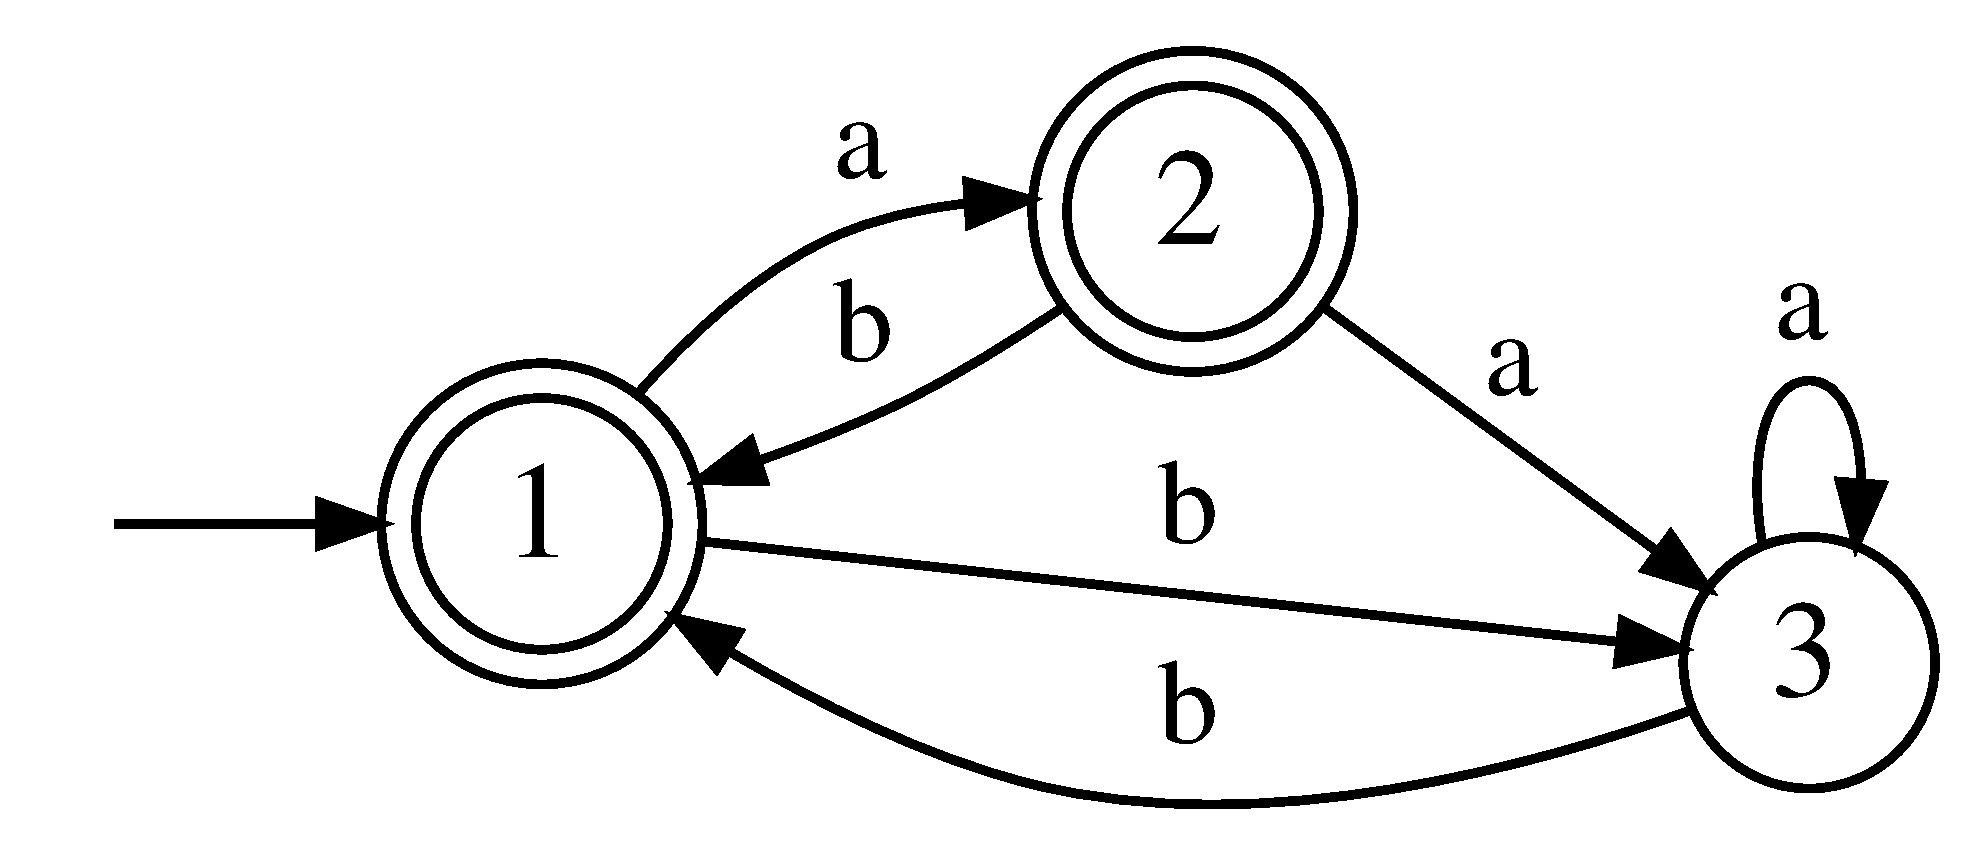
\includegraphics[scale=0.16]{img/datamod/FIG1.eps}
  \caption{Пример ДКА минимального размера, соответствующего наборам примеров поведения $S_{+} = \{aba, bb, bba\}$ и $S_{-} = \{b, ba\}$}
  \label{img:dfa-ex}
\end{figure}

\subsection{Расширенное префиксное дерево}
\label{sec:review:sat-dfa-inf:apta}

\inote{переписать начало}

Первым шагом большинства существующих подходов является построение \emph{расширенного префиксного дерева} (augmented prefix tree acceptor~{---} APTA) по имеющимся множествам примеров поведения $S_{+}$ и $S_{-}$. 
Расширенное префиксное дерево~--- это древовидная структура данных, основанная на обычном префиксном дереве (бор, нагруженное дерево, prefix tree, trie), отличающаяся от нее метками вершин.
Более формально, префиксным деревом называется шестерка $\mathcal{T} = \left(T,\Sigma,\tau,t_{1},T^{+}, T^{-}\right)$, где $T$~{---} конечное множество вершин, $\Sigma$~{---} алфавит входных символов, $\tau: T \times \Sigma \pto T$~{---} \emph{функция переходов}, $t_{1}$~{---} \emph{корневая} вершина (\emph{корень}), $T^{+} \subset T$~{---} множество \emph{допускающих} (\emph{принимающих}) вершин, $T^{-} \subset T$~{---} множество \emph{не допускающих} (\emph{отвергающих}) вершин.
В отличие от функции переходов в ДКА, функция переходов $\tau$ является частичной. 
Также, в префиксном дереве $T^{+} \cup T^{-} \subset T$, то есть некоторые вершины могут не являться ни принимающими, ни отвергающими~--- промежуточные вершины.

Расширенное префиксное дерево для множеств примеров поведения $S_{+}$ и $S_{-}$ строится как обычное префиксное дерево, но терминальные вершины для каждого слова помечаются соответствующей меткой. Вершины, в которых не заканчивается ни один из примеров поведения, остаются непомеченными. Пример расширенного префиксного дерева приведен на рисунку~\ref{img:apta-ex}.
Также далее в диссертации с помощью $\Delta(v)$ будет обозначаться расстояния от корневой вершины $t_{1}$ до вершины $t_{v}$.

\begin{figure}[ht]
  \centering
  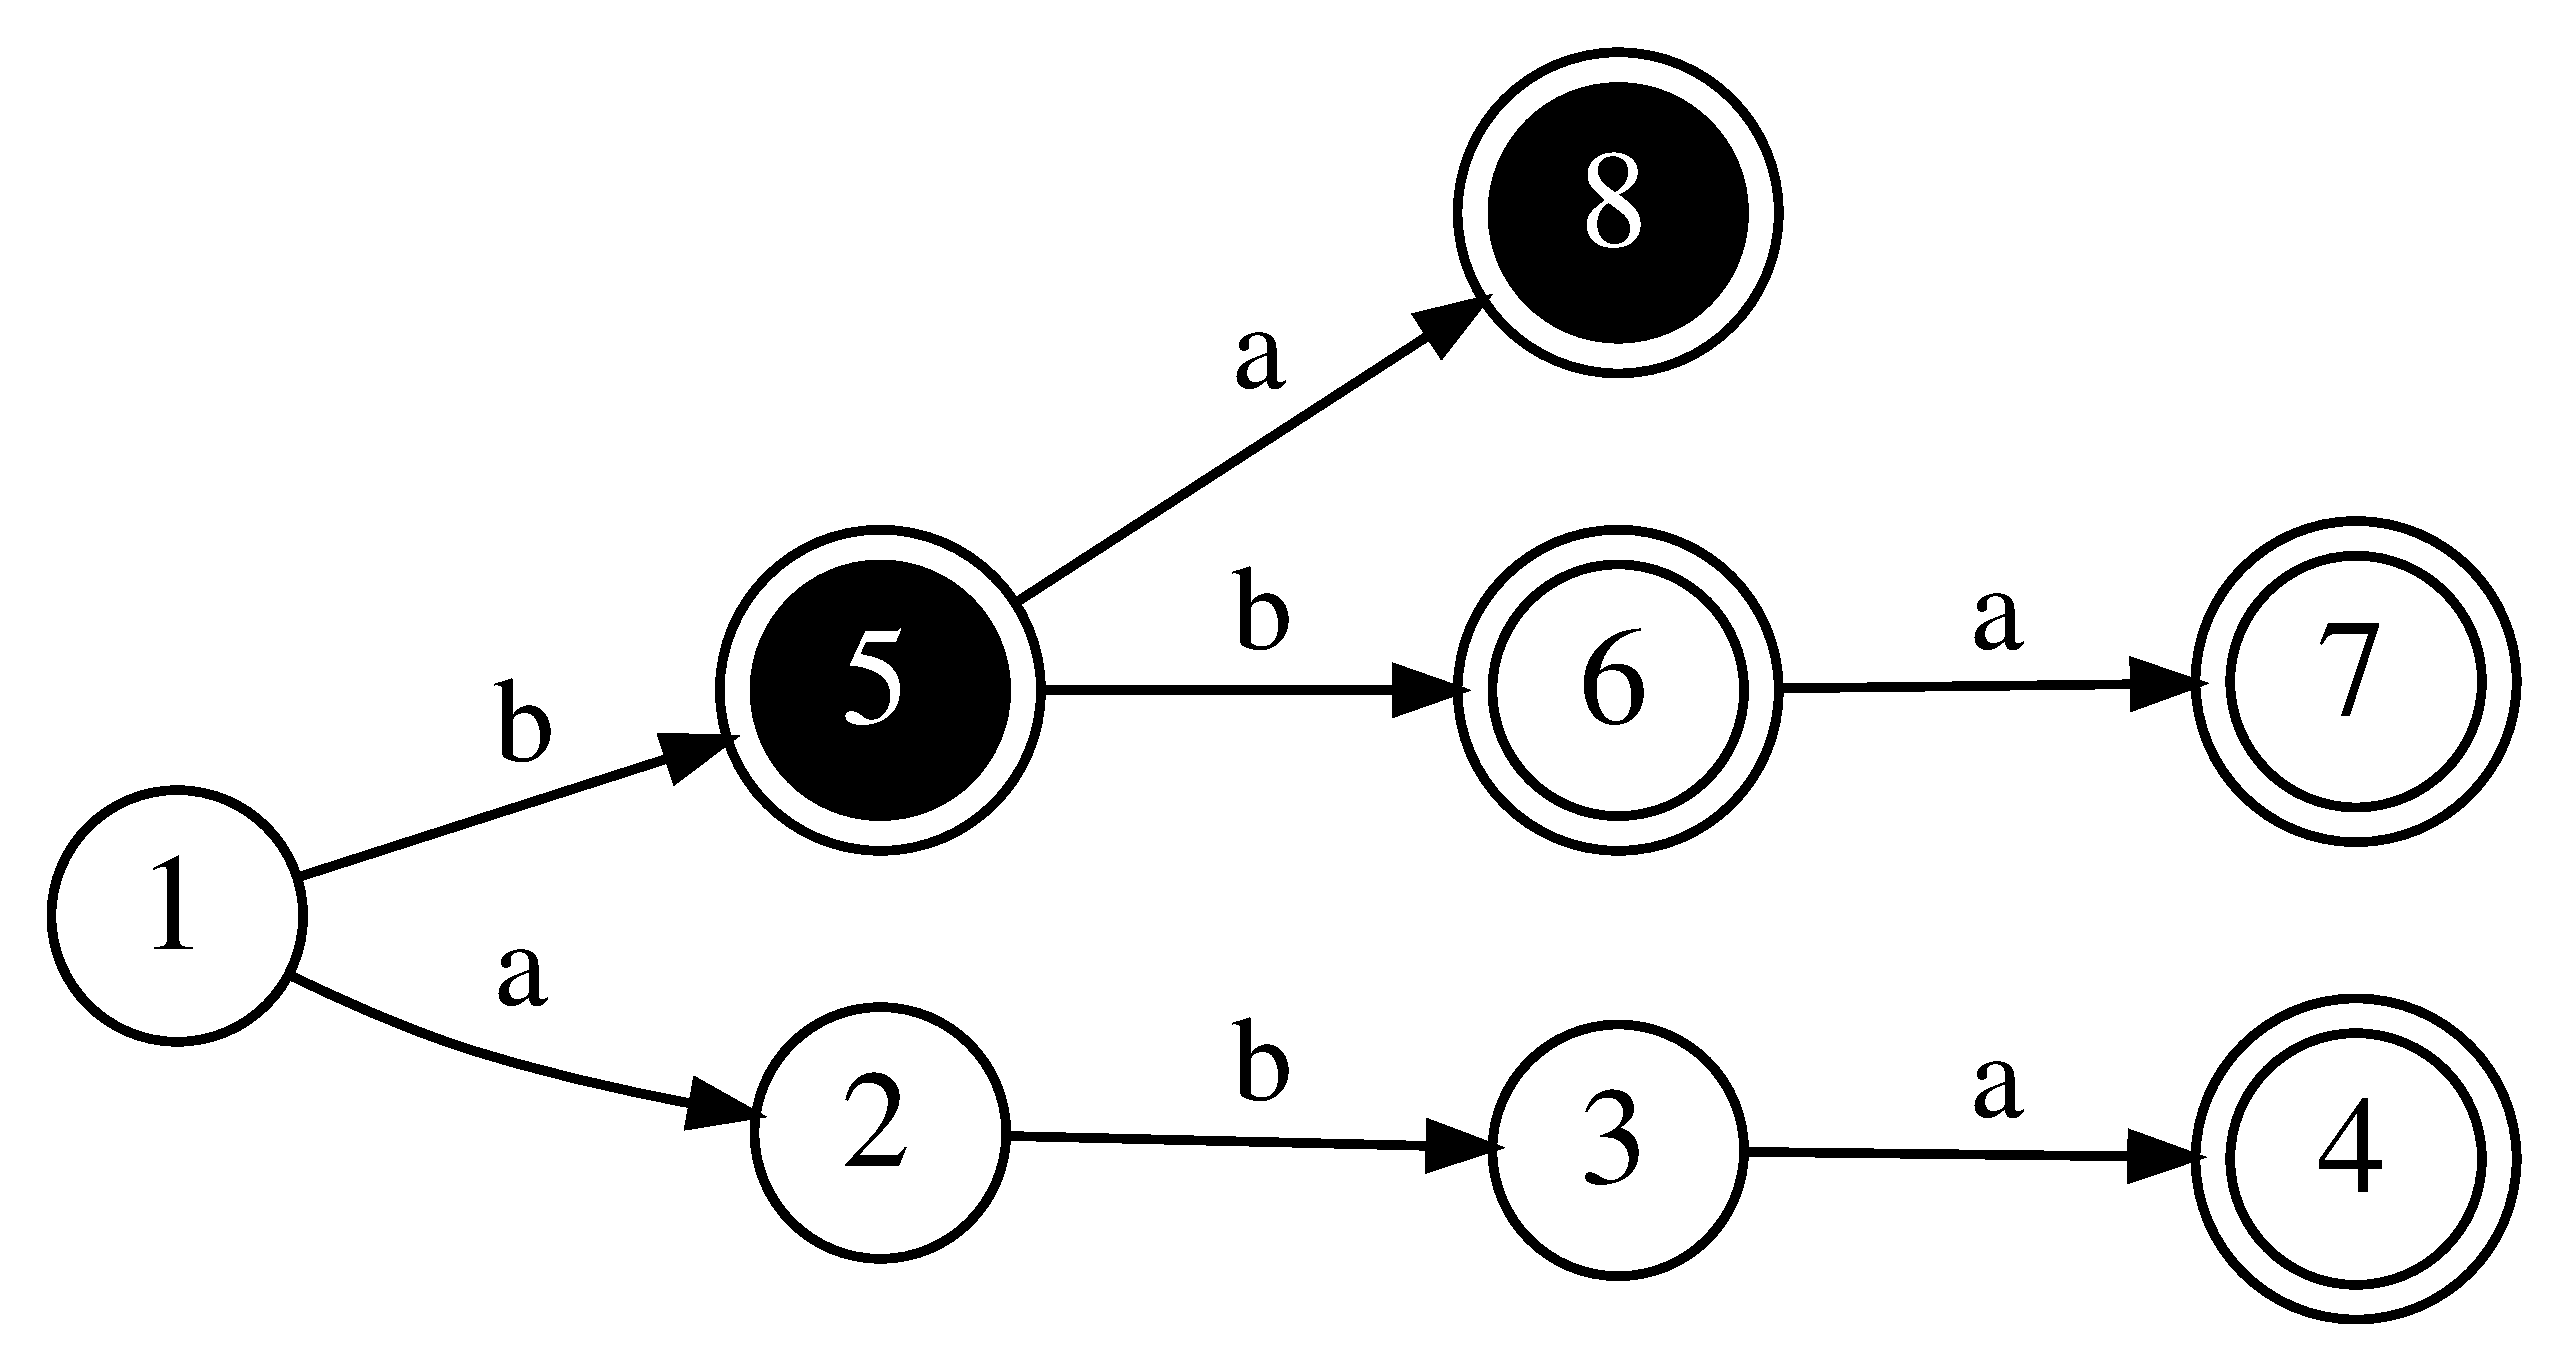
\includegraphics[scale=0.14]{img/datamod/FIG2a.eps}
  \caption{Пример расширенного префиксного дерева, построенного по наборам примеров поведения $S_{+} = \{aba, bb, bba\}$ и $S_{-} = \{b, ba\}$}
  \label{img:apta-ex}
\end{figure}

%----------------------------------------------------------------------------------------

\section{Эвристические и метаэвристические методы генерации детерминированных конечных автоматов} 
\label{sec:review:heuristic-dfa-inf}

В настоящем разделе приводится обзор существующих эвристических и метаэвристических методов генерации ДКА минимального размера по заданным примерам поведения.
Отличительной особенностью таких методов является то, что они не являются точными~--- ими не гарантируется, что какой-то ДКА будет найден в принципе, а если ДКА найден, то не гарантируется его минимальность.
Несмотря на то, что настоящая диссертация посвящена расширению границ применимости точных методов генерации ДКА, для построения достаточно больших автоматов по большому числу примеров поведения неточные эвристические и метаэвристические методы все еще являются единственным возможным вариантом.

\subsection{Эвристические алгоритмы}
\label{sec:review:heuristic-dfa-inf:heuristic}

В основе эвристических алгоритмов лежит идея \emph{слияния состояний} (\emph{state merging})~--- последовательных объединения вершин расширенного префиксного дерева (смотри раздел~\ref{sec:review:sat-dfa-inf:apta}) и устранения образующейся недетерминированности.
Самым успешным эвристическим алгоритмом можно считать алгоритм \emph{объединения состояний на основе свидетельств} (\emph{evidence-driven state merging}~--- EDSM)~\cite{DBLP:conf/icgi/LangPP98}.

\inote{требуется сильно дописать}

\subsection{Метаэвристические алгоритмы}
\label{sec:review:heuristic-dfa-inf:metaheuristic}

Среди метаэвристических алгоритмов, успешно применяемых для генерации конечных автоматов по примерам поведения, можно выделить эволюционные стратегии~\cite{DBLP:journals/pami/LucasR05,DBLP:conf/cec/Gomez06}, генетические алгоритмы~\cite{genetic-algs-dfa-inf-egorov-13} и муравьиные алгоритмы~\cite{chivilikhin-phd-15}.

\inote{требуется сильно дописать}


%----------------------------------------------------------------------------------------

\section{Методы генерации детерминированных конечных автоматов, основанные на сведении к другим NP-трудным задачам} 
\label{sec:review:sat-dfa-inf} 

В настоящем разделе приводится обзор существующих точных методов генерации ДКА по заданным примерам поведения при помощи сведения к задачам раскраски графа и выполнимости булевой формулы.

Лучшие эвристики выбора пары состояний для слияния в алгоритме EDSM обычно основаны на успешных эвристиках для других гораздо более активно изучаемых задач, например, для задачи выполнимости или задачи раскраски графа.
Как уже говорилось, ежегодно проходят соревнования по определению лучшего программного средства для решения SAT~\cite{sat-competitions}.
Несмотря на то, что различные эвристические стратегии выбора вершин для слияния повышают производительность метода EDSM и при его реализации используются оптимизированные структуры данных, данные реализации все еще значительно проигрывают по эффективности программным средствам для решения более проработанных задач.
Так как задача генерации ДКА является NP-полной~\cite{DBLP:journals/iandc/Gold78}, то ее можно свести к задачам, которые изучаются дольше и интенсивнее, чтобы использовать максимально оптимизированные стратегии поиска решения.

\subsection{Сведение к задаче раскраски графа}
\label{sec:review:sat-dfa-inf:coloring}

В работе французских ученых Косте и Николя~\cite{Coste97regularinference} предлагается сведение задачи генерации ДКА по заданным примерам поведения к задаче раскраски графа.
На первом шаге алгоритма как и ранее строится расширенное префиксное дерево по заданным примерам поведения.
Основной идей предложенного сведения является использование различных цветов для каждого из состояний генерируемого ДКА.
Раскраска производится таким образом, что, если все вершины расширенного префиксного дерева, соответствующие одному цвету в раскрашиваемом графе, объединить в одно состояние автомата, и проделать данную операцию для всех цветов, то в итоге должен получиться детерминированный конечный автомат. 

Ситуация, когда объединяются допускающая и отвергающая вершины графа, называется \emph{конфликтом}, так как состояние ДКА может быть только либо допускающим, либо отвергающим.
Очевидно, что тогда две вершины соединены ребром, если одна из них помечена как допускающая, а другая как отвергающая, так как их объединение приводит к конфликту.
Использование расширенного префиксного дерева, в котором существуют вершины, помеченные как промежуточные (то есть не являющиеся ни принимающими, ни отвергающими), позволяет в явном виде находить некоторые конфликты, которые возникают при объединении двух вершин, одна или две из которых являются промежуточными.
Объединение двух вершин расширенного префиксного дерева в одну может привести к недетерминированности~--- для новой вершины будет существовать несколько исходящих переходов, помеченных одним символом.
Избавиться от недетерминированности можно рекурсивно объединив вершины, куда ведут такие переходы.
Такой процесс называется \emph{детерминизацией}.
Если в процессе детерминизации возникает конфликт, то можно утверждать, что слияние вершин, объединенных на каждом из предыдущих шагов, приводит к конфликту.

Тогда, отметив в графе все найденные конфликты, можно перейти к решению задачи раскраски графа в $k$ цветов.
Так как исходная задача заключается в поиске ДКА с минимальным числом состояний, то требуется найти минимальное $k$ для которого существует правильная раскраска.
Добиться этого предлагается путем итеративного перебора числа цветов $k$, начиная с единицы и до тех пор, пока не будет найдено решение.

\inote{оставить только одно описание из двух}
\inote{рисунки красивые и цветные}

\subsection{Сведение к задаче выполнимости}
\label{sec:review:sat-dfa-inf:sat}

Как было сказано в разделе~\ref{sec:review:sat:methods}, программные средства для решения задачи выполнимости в последние несколько десятилетий~--- фактически с 1996 года, когда был предложен алгоритм CDCL~--- сильно развились и стали достаточно мощными средствами для решения многих прикладных задач, выраженных на языке SAT.
Например, сведение к SAT используется для решения таких задач, как символьная проверка моделей~\cite{DBLP:conf/tacas/BiereCCZ99}, поиск связей между различными контекстами в распределенных системах~\cite{DBLP:conf/context/BouquetMSZ03}, поиск ошибок в программах на языке программирования \texttt{C}~\cite{DBLP:conf/cav/XieA05}, поиск кратчайшего синхронизирующего слова~\cite{DBLP:conf/wia/SkvortsovT11}, кластеризация в ограничения~\cite{DBLP:conf/ida/MetivierBCKL12}, генерация оптимальных деревьев решений~\cite{DBLP:conf/ijcai/NarodytskaIPM18} и множества других.

В 2010 году в статье~\cite{heule-icgi10} учеными Марейном Хойлом (Marijn Heule) и Сикко Вервером (Sicco Verwer) впервые был предложен метод генерации ДКА по заданным примерам поведения, основанный на сведении к задаче выполнимости, названный DFASAT.
Метод DFASAT основан на описанном в предыдущем разделе сведении задачи генерации ДКА к задаче раскраски графа.
Существует широко известное сведение задачи раскраски графа к SAT, которое Хойл и Вервер называют \emph{прямым кодированием} (\emph{direct encoding})~\cite{DBLP:conf/cp/Walsh00}.
Однако, авторы показывают, что использование прямого кодирования для задачи генерации ДКА приводит к построению булевой формулы, состоящей из $\mathcal{O}\left(N^{2} \times M^{2}\right)$, где $N$~--- размер префиксного дерева, $M$~--- размер генерируемого автомата, дизъюнктов.
Для нетривиальных примеров задачи генерации ДКА формула такого сложности получается слишком большой для современных программных средств для решения SAT, поэтому авторы предложили \emph{компактное сведение} (\emph{compact encoding}).

Здесь, и далее в диссертации, используется следующее обозначение: $\left[N\right] = {1,2,\ldots,N}$.
Для компактного сведения необходим ввести три типа булевых переменных:
\begin{enumerate}
  \item переменные соответствия $\{x_{v,i}\}_{v \in T, i \in \left[M\right]}$, которые истинны тогда и только тогда, когда вершина $t_{v}$ в расширенном префиксном дереве $\mathcal{T}$ соответствует состоянию $d_{i}$ в автомате $\mathcal{D}$;
  \item переменные перехода $\{y_{i,l,j}\}_{i,j \in \left[M\right],l \in \Sigma}$, которые истинны тогда и только тогда, когда в автомате $\mathcal{D}$ существует переход из состояния $d_{i}$ в состояние $d_{j}$ по символу $l$;
  \item переменные допуска $\{z_{i}\}_{i \in \left[M\right]}$, которые истинны тогда и только тогда, когда в автомате $\mathcal{D}$ состояние $d_{i}$ является допускающим.
\end{enumerate}

Используя вышеопределенные переменные, компактное сведение, представляется с помощью следующих множеств дизъюнктов.

\inote{ОПА. Только что осознал, что так как половина из этих дизъюнктов является избыточными, необязательными, то они тоже служат для сокращения пространства поиска, а значит их надо, видимо, отдельно рассматривать. У Сикко и Хойла это называлось прямое сведение и какое-то там еще.}

\begin{enumerate}
  \item $\left(x_{v,1} \vee x_{v,2} \vee \ldots \vee x_{v,M}\right)$ для $v \in \left[N\right]$~{---} каждой вершине $t_{v}$ расширенного префиксного дерева $\mathcal{T} $ в соответствие ставится как минимум одно состояние автомата $\mathcal{D}$.
  %
  \item $\left(\neg y_{i,l,j} \vee \neg y_{i,l,h}\right)$ для $i,j,h \in \left[M\right]; j < h; l \in \Sigma$~{---} из каждого состояния $d_{i}$ автомата $\mathcal{D}$ существует не более одного перехода по каждому символу $l$ алфавита $\Sigma$, иными словами, ДКА $\mathcal{D}$ детерминирован.
  %
  \item $\left(\neg x_{v,i} \vee z_{i}\right)$ для $t_{v} \in T^{+}; i \in \left[M\right]$~{---} если принимающей вершине $t_{v}$ расширенного префиксного дерева $\mathcal{T}$ в соответствие ставится состояние $d_{i}$ автомата $\mathcal{D}$, то это состояние также должно быть принимающим.
  %
  \item $\left(\neg x_{v,i} \vee \neg z_{i}\right)$ для $t_{v} \in T^{-}; i \in \left[M\right]$~{---} если отвергающей вершине $t_{v}$ расширенного префиксного дерева $\mathcal{T}$ в соответствие ставится состояние $d_{i}$ автомата $\mathcal{D}$, то это состояние также должно быть отвергающим.
  %
  \item $\left(\neg x_{v,i} \vee \neg x_{w,j} \vee y_{i,l,j}\right)$ для $v,w \in \left[N\right]; i,j \in \left[M\right];l \in \Sigma; \tau\left(t_{v},l) = t_{w}\right)$~{---} если вершине $t_{v}$ расширенного префиксного дерева $\mathcal{T} $ в соответствие ставится состояние $d_{i}$ автомата $\mathcal{D}$, вершине $t_{w}$~{---} состояние $d_{j}$ и в префиксном дереве $\mathcal{T}$ существует переход из вершины $t_{v}$ в вершину $t_{w}$ по символу $l$, то в автомате $\mathcal{D}$ должен быть переход из состояния $d_{i}$ в состояние $d_{j}$ по символу $l$.
  %
  \item $x_{1,1}$~{---} корню $t_{1}$ расширенного префиксного дерева $\mathcal{T} $ в соответствие ставится начальное состояние $d_{1}$ автомата $\mathcal{D}$.
\end{enumerate}

\inote{симметри бреакинг дальше}

\begin{enumerate}
  \item $\left(\neg x_{v,i} \vee \neg x_{v,j}\right)$ для $v \in \left[N\right]; i,j \in \left[M\right]; i < j$~{---} каждой вершине $t_{v}$ расширенного префиксного дерева $\mathcal{T} $ в соответствие ставится не более одного состояния автомата $\mathcal{D}$.
  %
  \item $\left(y_{i,l,1} \vee y_{i,l,2} \vee \ldots \vee y_{i,l,M}\right)$ для $i \in \left[M\right]; l \in \Sigma$~{---} из каждого состояния $d_{i}$ автомата $\mathcal{D}$ существует как минимум один переход по каждому символу $l$ алфавита $\Sigma$, иными словами, ДКА $\mathcal{D}$ полон.
  %
  \item $\left(\neg x_{v,i} \vee \neg y_{i,l,j} \vee x_{w,j}\right)$ для $v,w \in \left[N\right]; i,j \in \left[M\right];l \in \Sigma; \tau\left(t_{v},l) = t_{w}\right)$~{---} если вершине $t_{v}$ расширенного префиксного дерева $\mathcal{T} $ в соответствие ставится состояние $d_{i}$ автомата $\mathcal{D}$, и в префиксном дереве $\mathcal{T}$ существует переход из вершины $t_{v}$ в вершину $t_{w}$ по символу $l$ и в автомате $\mathcal{D}$ существует переход из состояния $d_{i}$ в состояние $d_{j}$ по символу $l$, вершине $t_{w}$ дерева $\mathcal{T}$ должно ставиться в соответствие состояние $d_{j}$.
  %
\end{enumerate}

Все представленные выше наборы дизъюнктов могут быть объединены с помощью конкатенации в одну большую булеву формулу. Всего в такой формуле будет $\mathcal{O}(N \times M^{2})$ дизъюнктов и для их кодирования будет использовано $\mathcal{O}(M^2 + N \times M)$ переменных.

Схема метода \texttt{DFASAT} представлена на рисунке~\ref{img:dfasat-algo}.

\begin{figure}[ht]
  \centering
  \includegraphics[scale=0.7]{img/ntv/basic.jpg}
  \caption{Схема точного метода генерации ДКА по заданным примерам поведения на основе сведения к SAT~--- \texttt{DFASAT}}
  \label{img:dfasat-algo}
\end{figure}


%----------------------------------------------------------------------------------------

\section{Подходы к сокращению пространства поиска при генерации детерминированных конечных автоматов}
\label{sec:review:sym-breaking}

В настоящем разделе приводится обзор существующих подходов к сокращению пространства поиска при решении задачи выполнимости для генерации ДКА по заданным примерам поведения. 

\inote{рассказать про пространство поиска в принципе}

\subsection{Граф несовместимости}
\label{sec:review:sym-breaking:ig}

Помимо пропозиционального кодирования, описанного в разделе~\ref{sec:review:sat-dfa-inf}, авторы~\cite{heule-icgi10} предложили использовать вспомогательную структуру данных, названную ими \emph{графом совместимости} (\emph{consistency graph}).
Несмотря на оригинальное название, как будет видно далее, данная структура данных должна скорее называться \emph{графом несовместимости} (\emph{inconsistency graph}).
В данной диссертации предлагается использовать последнее название.

В основе данной идеи лежит подход со слияниями состояний.
Две вершины $t_{v}$ и $t_{w}$ расширенного префиксного дерева можно слить (объединить, merge) в одну вершину $t_{v'}$, объединив множества исходящих из них переходов.
Если в результате данной операции в префиксном дереве возникла недетерминированность, то есть из вершины $t_{v'}$ теперь исходят два различных перехода по одному и тому же символу в различные вершины $t_{q}$ и $t_{r}$, то от нее можно избавиться объединив вершины $t_{q}$ и $t_{r}$ в одну вершину $t_{q'}$. 
Рекурсивно продолжая данный процесс, можно избавиться от всех случаев недетерминированности в префиксном дереве.
Важным фактом является то, что если в процессе избавления от недетерминированности в какой-то момент приходится объединить принимающую вершину с отвергающей, то изначальное слияние вершин $t_{v}$ и $t_{w}$ невозможно.
В таком случае говорят, что вершины $t_{v}$ и $t_{w}$ \emph{несовместимы} (\emph{inconsistent}).
Данную информацию можно использовать для помощи программному средству для решения задачи SAT.

Более формально, по имеющемуся расширенному префиксному дереву $\mathcal{T} = \left(T,\Sigma,\tau,t_{1},T^{+},T^{-}\right)$ предлагается построить граф $\mathcal{I} = \left(V, E\right)$ такой, что его множество вершин $V$ совпадает со множеством вершин $\mathcal{T}$ префиксного дерева $\mathcal{T}$, а множество ребер $E$ определяется следующим образом. 
Две вершины в графе $\mathcal{I}$ соединены ребром тогда и только тогда, когда их объединение и последующее избавление от недетерминированности приводит к несовместимости. 

Так как искомый ДКА $\mathcal{D}$ соответствует префиксному дереву $\mathcal{T}$, то если две вершины $t_{v}$ и $t_{w}$ смежны в графе несовместимости $\mathcal{I}$, то они не могут соответствовать одному и тому же состоянию $d_{i}$ автомата $\mathcal{D}$.
Данное свойство может быть выражено с помощью переменных $x_{v,i}$ в виде следующего множества дизъюнктов~{---} $\left(\neg x_{v,i} \vee \neg x_{w,i}\right)$ для $v,w \in \left[N\right]; \left(v,w\right) \in E; i \in \left[M\right]$.
Такие дизъюнкты необязательны, но их добавление к основной булевой формуле помогает значительно сократить пространство поиска программного средства для решения SAT. 
Однако, надо заметить, что в общем случае таких дизъюнктов будет $\mathcal{O}\left(N^{2} \times M\right)$, что на порядок относительно $N$ увеличивает размер формул. 
Использование графа несовместимости в таком виде для построения больших автоматов по большому множеству примеров поведения нецелесообразно. 
% В разделе \inote{ДОБАВИТЬ ССЫЛКУ} будут предложены несколько способов использования только части графа несовместимости, что не увеличивает размер формулы, но позволяет дополнительно сократить пространство поиска.

\subsection{Изоморфные автоматы}
\label{sec:review:sym-breaking:isomorphic-automata}


При решении многих задач комбинаторной оптимизации, коей фактически является задача генерации ДКА минимального размера, зачастую существуют симметричные решения (симметрии)~\cite{DBLP:conf/aaai/Walsh12}.
Симметрии увеличивают пространство поиска и, таким образом, значительная часть времени тратится на проверку новых решений, которые симметричны уже просмотренным.
В задаче генерации ДКА по примерам поведения такой симметрией являются изоморфные автоматы.
Автоматы называются \emph{изоморфными} если существует биекция между их состояниями такая, что сохраняются все переходы, принимающие состояния соответствуют принимающим, а начальное~--- начальному.
Иными словами, автоматы являются изоморфными, если они различаются только нумерацией состояний, но не своей структурой.
Тогда можно сделать вывод, что число изоморфных автоматов можно оценить с помощью числа перестановок.
Таким образом, для некоторого ДКА $\mathcal{D}$ c $M$ состояниями существует $\mathcal{O}\left(M!\right)$ изоморфных ему ДКА.

\inote{Возможно, дописать еще что-то + рисунки}

\subsection{Большая клика}
\label{sec:review:sym-breaking:large-clique}

Как было сказано в предыдущем разделе, при отсутствии каких-либо ограничений на нумерацию состояний автомата, существует $M!$ изоморфных автоматов.
Авторы~\cite{heule-icgi10} предложили свой способ нарушения симметрии, позволяющий сократить число рассматриваемых изоморфных автоматов.
Так как в графе несовместимости смежные вершины по определению не могут соответствовать одному состоянию в искомом ДКА, то все вершины в некоторой клике (клика~{---} полный граф, граф в котором каждая вершина соединена ребром со всеми остальными) \inote{ссылку на статью про клики} такого графа будут соответствовать различным состояниям автомата.
Учитывая, что итоговая нумерация состояний автомата не важна, можно, не уменьшая общности, зафиксировать номера вершин такой клики, что и было предложено в рассматриваемой статье.

Однако, задача поиска клики максимального размера в некотором графе является NP-полной~\cite{DBLP:conf/coco/Karp72}.
Поэтому авторами было предложено найти клику большого, но не обязательно максимального размера.
Сделать это можно с помощью следующего эвристического подхода.
В графе ищется вершина максимальной степени, которая будет входить в искомую большую клику.
Затем ищется смежная ей вершина максимальной степени и добавляется в клику.
Затем ищется вершина максимальной степени смежная обеим предыдущим и также добавляется в клику. 
Повторяя данный процесс, пока есть возможность существуют вершины смежные всем уже добавленным в клику.

Таким образом, если размер найденной клики равен $C$, то вместо $M!$ изоморфных автоматов будут рассмотрены $(M - C)!$ изоморфных автомата.
Учитывая скорость роста факториала, разница между $M!$ и $(M - C)!$ может быть значительной, однако в общем случае число рассматриваемых изоморфных автоматов все еще остается факториальным относительно размера автомата.
Помимо вышеуказанного недостатка, данный подход требует обязательного построения полного графа несовместимости, что, как было/будет \inote{???} рассмотрено ранее/далее, далеко не всегда является возможным.

\subsection{Предикаты нарушения симметрии на основе алгоритма обхода графа в ширину}
\label{sec:review:sym-breaking:bfs-based}

Идеальным нарушением симметрии является ситуация, когда для каждого класса эквивалентности относительно симметрии остается единственный представитель. 
Для задачи генерации ДКА~{---} когда для каждого класса эквивалентности по изоморфизму остается единственный представитель.
Автором данной диссертации совместно с научным руководитем \inote{тут понять как статью с первой латы обыгрывать} в~\cite{zakirzyanov2015LATA} были разработаны предикаты нарушения симметрии на основе алгоритма обхода графа в ширину, которые позволяют добиться идеального нарушения симметрии

Идея предложенного подхода состоит в том, чтобы зафиксировать нумерацию состояний в порядке \emph{обхода в ширину} (\emph{breadth-first search}~{---} BFS) данного автомата.
\inote{наверное, нужно рассказать, что за BFS такой. описание+псевдокод}
Для того, чтобы сделать обход в ширину уникальным, необходимо зафиксировать некоторый порядок на входных символах переходов, например, лексикографический. 
Будем называть ДКА \emph{BFS-пронумерованным}, если нумерация его состояний соответствует порядку обхода его состояний в ширину.
Тогда в каждом классе эквивалентности по изоморфизму будет ровно один BFS-пронумерованный представитель.

Другими словами, если рассмотреть дерево BFS, построенное для некоторого ДКА, расположив при этом детей в соответствии с выбранным порядком на символах переходов, тогда номера состояний:
\begin{itemize}
  \item должны быть различными числами от $1$ до $M$;
  \item на одной глубине должны увеличиваться слева направо (\emph{порядок по уровню});
  \item должны увеличиваться сверху вниз (\emph{порядок по глубине}).
\end{itemize}
Пример BFS-пронумерованного автомата представлен на рисунке~\ref{img:bfs-ex}.
На рисунке~\ref{img:bfs-tree-ex} представлено соответствующее ему BFS-дерево.

\begin{figure}[ht]
  \centering
  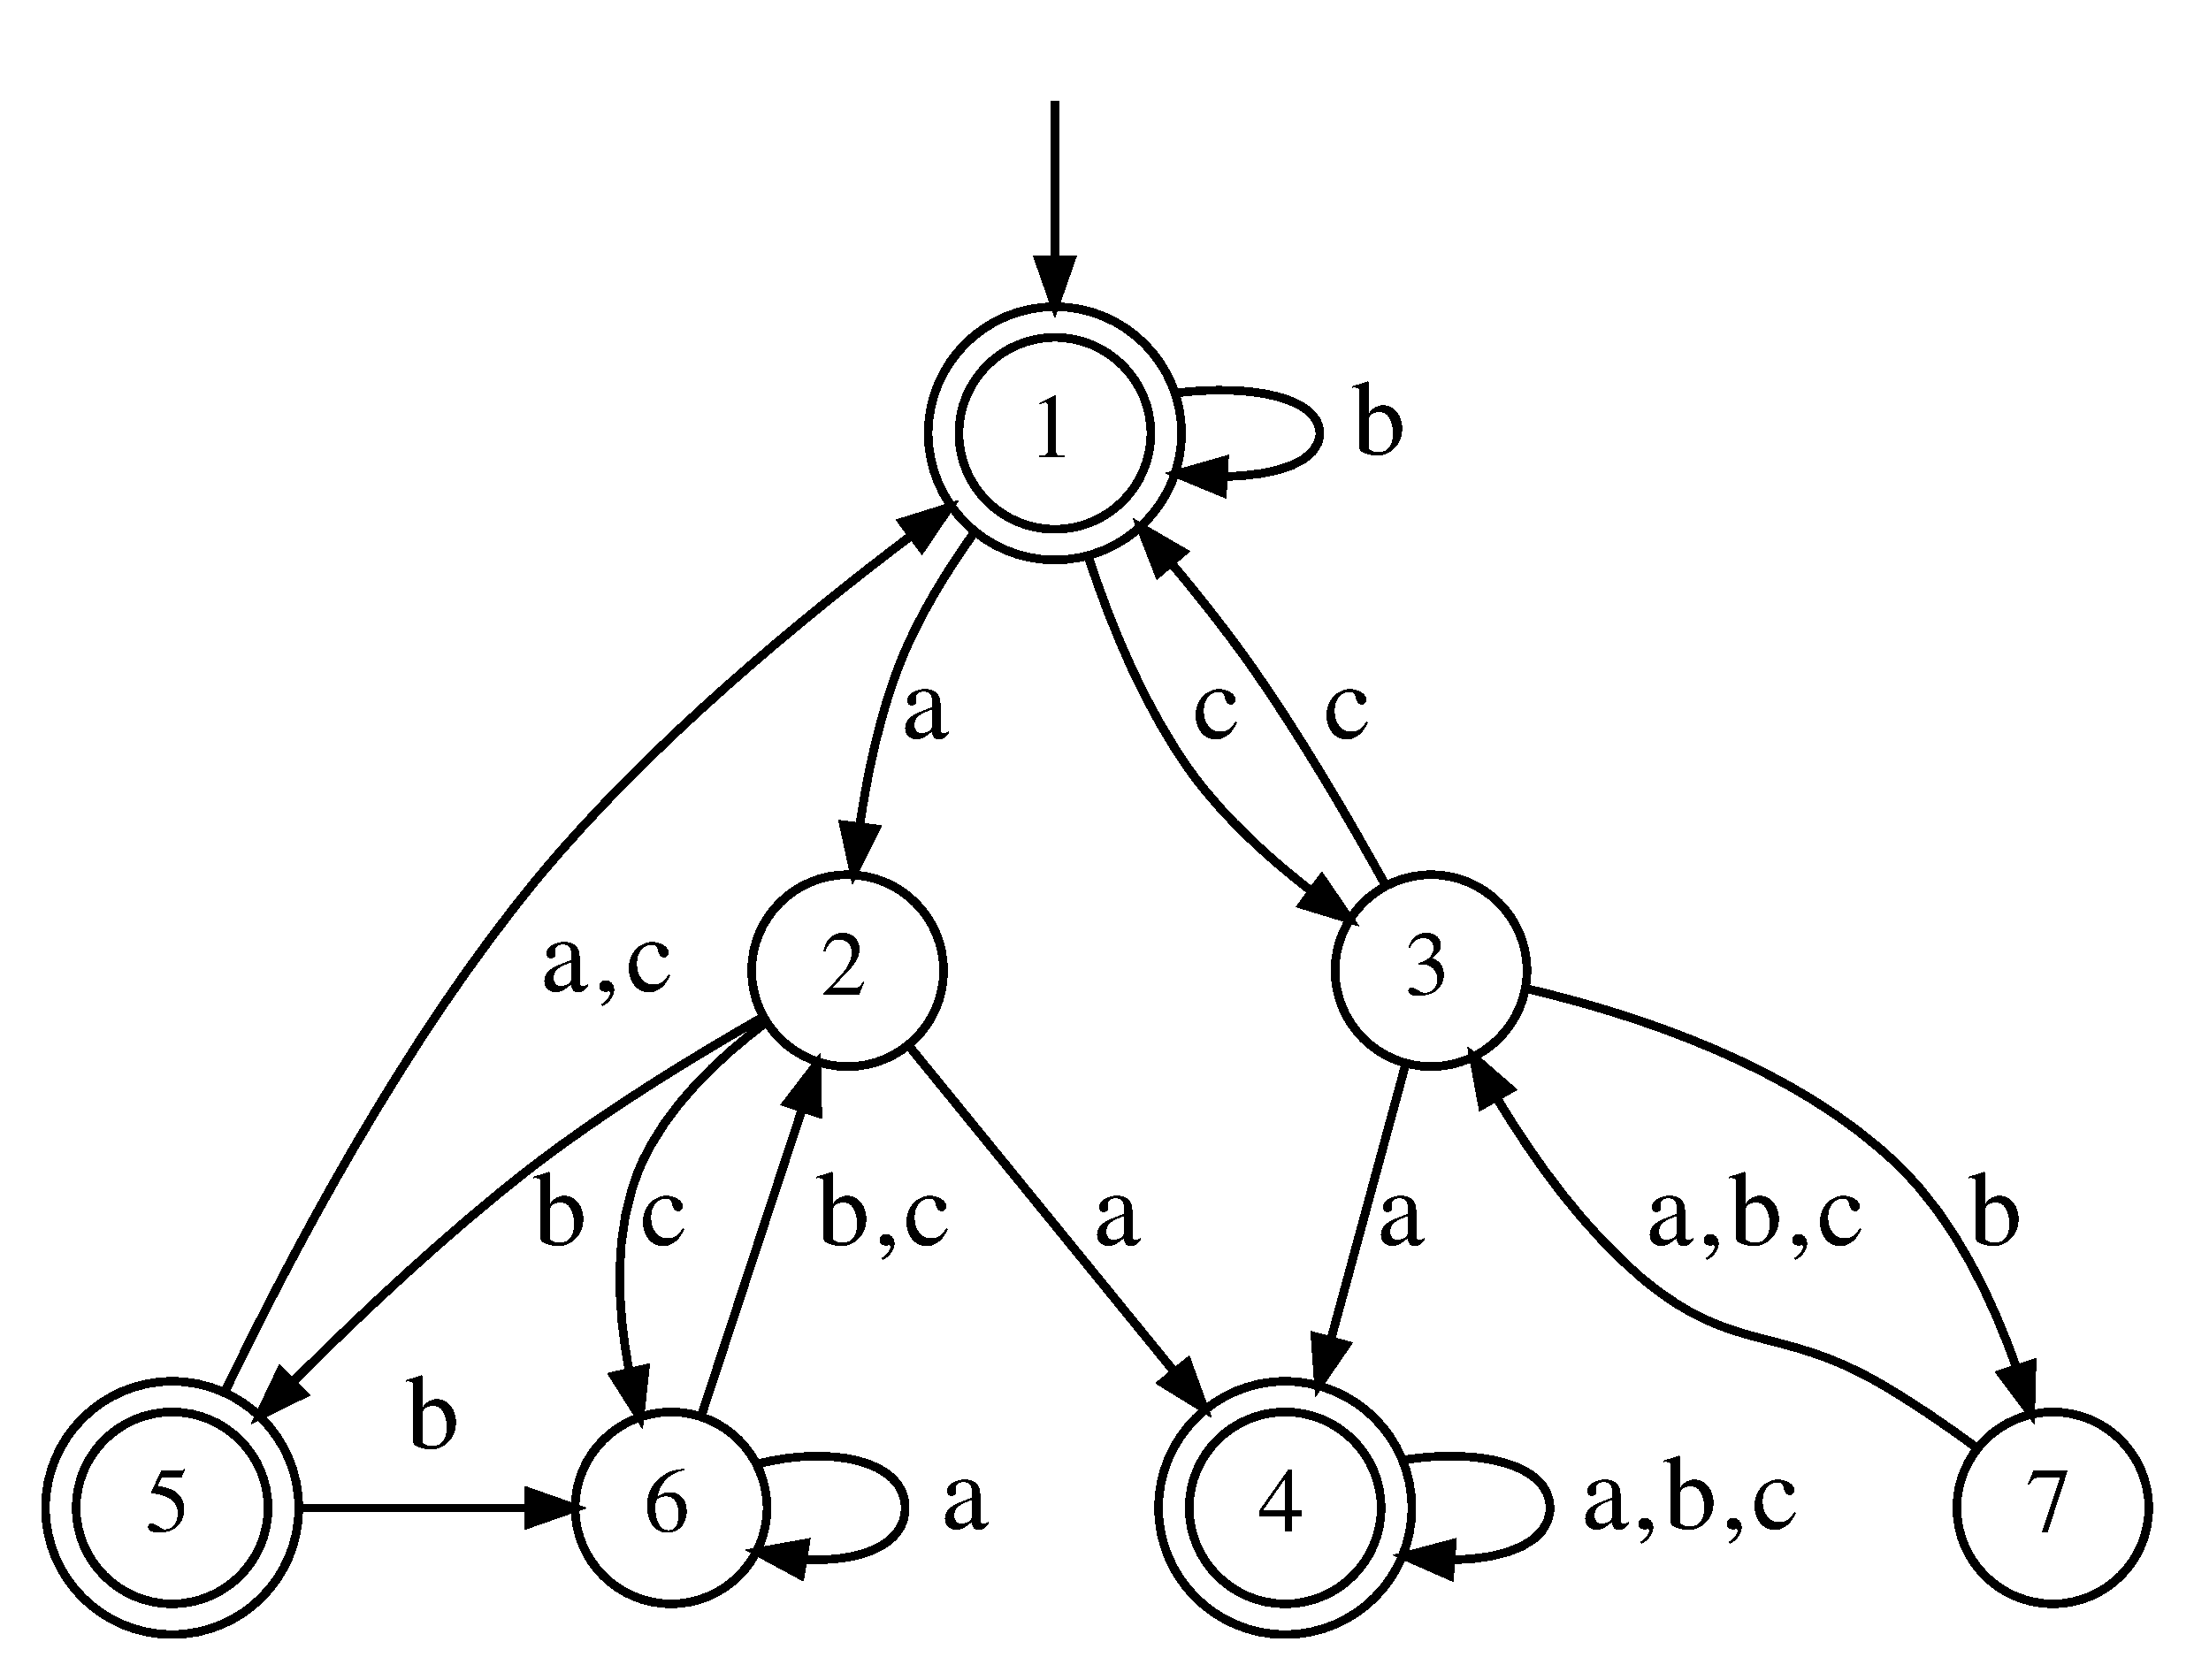
\includegraphics[scale=0.15]{img/datamod/BFS-example.eps}
  \caption{Пример BFS-пронумерованного автомата}
  \label{img:bfs-ex}
\end{figure}

\begin{figure}[ht]
  \centering
  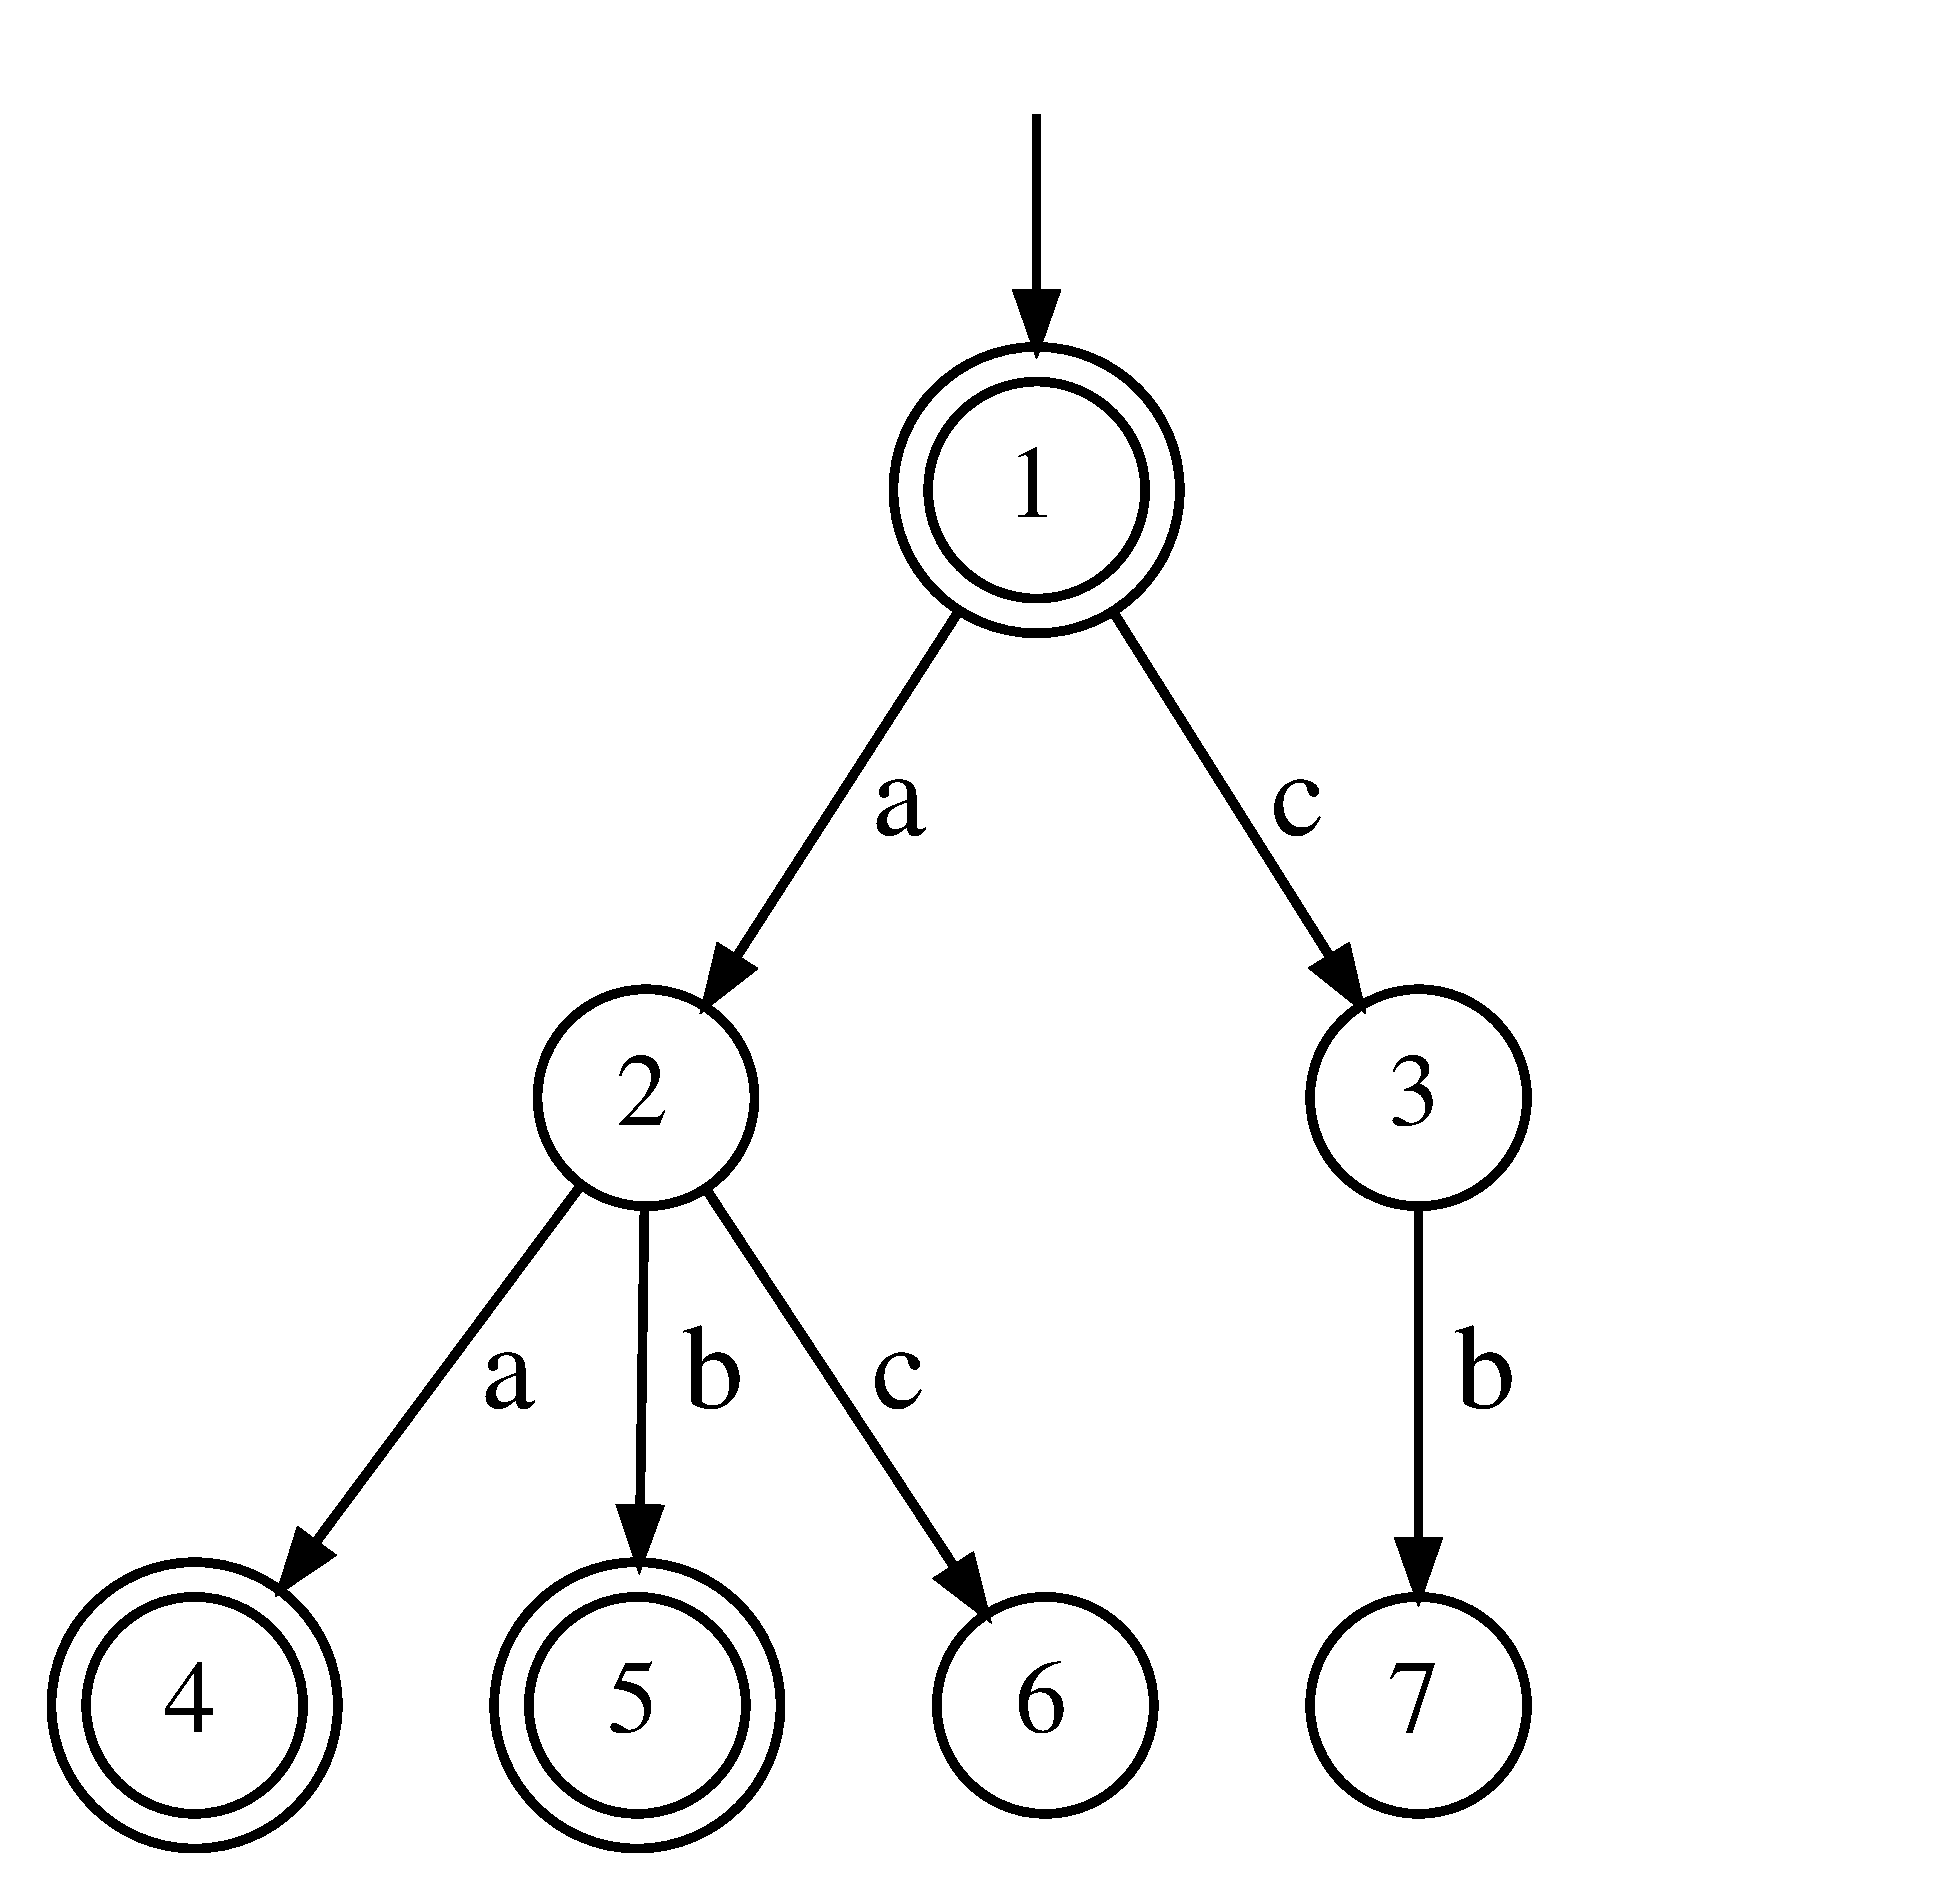
\includegraphics[scale=0.15]{img/datamod/BFS-tree.eps}
  \caption{BFS-дерево для автомата, представленного на рисунке~\ref{img:bfs-ex}}
  \label{img:bfs-tree-ex}
\end{figure}

Если закодировать требование к автомату, чтобы он был BFS-пронумерованным, в виде булевых предикатов и добавить к имеющейся формуле, предложенной в~\cite{heule-icgi10}, то программное средство для решения SAT будет искать автоматы, удовлетворяющие заданным примерам поведения, пронумерованные в порядке BFS.
Для того, чтобы закодировать данное требование, было предложено ввести три новых типа булевых переменных:

\begin{enumerate}
  \item переменные родителей $\{p_{j,i}\}_{1 \leq i < j \leq M}$, которые истинны тогда и только тогда, когда состояние $d_i$ является родителем состояния $d_j$ в BFS-дереве автомата $\mathcal{D}$;
  \item переменные наличия переходов $\{t_{i,j}\}_{1 \leq i < j \leq M}$, которые истинны тогда и только тогда, когда в автомате $\mathcal{D}$ существует переход из состояния $d_{i}$ в состояние $d_{j}$;
  \item переменные минимального символа $\{m_{i,l,j}\}_{1 \leq i < j \leq M;l \in \Sigma}$, которые истинны тогда и только тогда, когда в автомате $\mathcal{D}$ из состояния $d_{i}$ в состояние $d_{j}$ существует переход по символу $l$, но не существует переходов по меньшим (согласно выбранному порядку на символах) символам.
  Данные переменные используются только в случае небинарного алфавита.
\end{enumerate}

Используя данные переменные, можно закодировать свойство BFS-пронумерованности автомата с помощью следующих множеств дизъюнктов.

\begin{enumerate}
  \item $\left(t_{i,j} \leftrightarrow y_{i,l_{1},j} \vee y_{i,l_{2},j} \vee \ldots \vee y_{i,l_{L},j} \right)$ для $1 \leq i < j \leq M; l_{k} \in \Sigma$~--- в автомате $\mathcal{D}$ переход из состояния $d_{i}$ в состояние $d_{j}$ существует тогда и только тогда, когду существует переход из состояния $d_{i}$ в состояние $d_{j}$ хотя бы по одному из символов алфавита $\Sigma$.
  
  \item $\left(p_{j,i} \leftrightarrow t_{i,j} \wedge \neg t_{i - 1,j} \wedge \neg t_{i - 2, j} \wedge \ldots \wedge \neg t_{1,j}\right)$ для $1 \leq i < j \leq M$~{---} состояние $d_{i}$ автомата $\mathcal{D}$ является родителем состояния $d_{j}$ в BFS-дереве, если из состояния $d_{i}$ существует переход в состояние $d_{j}$, а из состояний с меньшим номером такого перехода не существует.
  
  \item $\left(p_{j,1} \vee p_{j,2} \vee \ldots \vee p_{j,j - 1}\right)$ для $2 \leq j \leq M$~{---} у каждого состояния $d_{j}$ автомата $\mathcal{D}$, кроме стартового, родитель в BFS-дереве должен иметь меньший номер. 
  Данные дизъюнкты позволяют закодировать порядок по глубине в поддереве.

  \item $\left(p_{j,i} \rightarrow \neg p_{j + 1, k}\right)$ для $1 \leq k < i < j \leq M$~{---} если состояние $d_{i}$ является родителем в дереве BFS состояния $d_{j}$, то у состояния с б\emph{о}льшим номером $d_{j + 1}$ родитель не может иметь номер меньший, чем $i$. 
  Данные дизъюнкты позволяют задать порядок по уровню для детей различных родителей, а также порядок по глубине в разных поддеревьях.
  
  \item $\left(p_{j,i} \wedge p_{j + 1, i} \rightarrow y_{i,l_{1},j}\right)$ для $1 \leq i < j \leq M;\Sigma=\{l_{1},l_{2}\}$~{---} если состояние $d_i$ является родителем в дереве BFS двух состояний $d_{j}$ и $d_{j+1}$ и алфавит бинарный, то переход из состояния $d_{i}$ в $d_{j}$ должен быть по меньшему символу.
  В случае бинарного алфавита данного множества дизъюнктов достаточно, чтобы упорядочить двух детей $d_{j}$ и $d_{j + 1}$ одного состояния $d_{i}$. 
  Дополнительно, для сокращения пространства поиска, можно добавить множество дизъюнктов $\left(p_{j,i} \wedge p_{j + 1, i} \rightarrow y_{i,l_{2},j + 1}\right)$ для $1 \leq i < j \leq M$. 
  Данные дизъюнкты задают порядок по уровню для детей одного родителя в случае бинарного алфавита.

  \item $\left(m_{i,l_{n},j} \leftrightarrow y_{i,l_{n},j} \wedge \neg y_{i,l_{n - 1}, j} \wedge \neg y_{i,l_{n - 2}, j} \wedge \ldots \wedge \neg y_{i,l_{1},j} \right)$ для $1 \leq i < j \leq M; 1 \leq n \leq L;l_{n} \in \Sigma$~{---} в автомате $\mathcal{D}$ символ $l_{n}$ является минимальным символом на переходах из состояния $d_{i}$ в состояние $d_{j}$ тогда и только тогда, когда в автомате существует переход из состояния $d_{i}$ в состояние $d_{j}$ по символу $l_{n}$, но не существует переходов по меньшим (относительно выбранного порядка) символам.
  Данное множество дизъюнктов используется в случае небинарного алфавита.

  \item $\left(p_{j,i} \wedge p_{j + 1, i} \wedge m_{i,l_{n}, j} \rightarrow \neg m_{i, l_{k}, j + 1}\right)$ для $1 \leq i < j \leq M; 1 \leq k < n \leq L;l_n,l_k \in \Sigma$~{---} если состояние $d_{i}$ является родителем в дереве BFS двух состояний $d_{j}$ и $d_{j + 1}$ и алфавит состоит из более чем двух символов, то из состояния $d_{i}$ переход в состояние $d_{j}$ должен быть по меньшему (относительно выбранного порядка) символу чем в состояние $d_{j + 1}$.
  Данные дизъюнкты задают порядок по уровню для детей одного родителя в случае небинарного алфавита.
\end{enumerate}

Все представленные выше наборы дизъюнктов могут быть объединены с помощью конкатенации в одну большую булеву формулу. Всего в такой формуле будет $\mathcal{O}(M^{3} + M^{2} \times L^{2})$ дизъюнктов и для их кодирования будет использовано $\mathcal{O}(M^2 \times L)$ переменных.

%----------------------------------------------------------------------------------------

\section{Подход уточнения абстракции по контрпримерам}
\label{sec:review:cegar}

Впервые метод \emph{уточнения абстракции по контрпримерам} (counterexample-guided abstraction refinement~--- CEGAR) был предложен в 2000 году Эдмундом Кларком и коллегами~\cite{DBLP:conf/cav/ClarkeGJLV00}.
Изначально данный метод был разработан для автоматизированного итеративного построения абстрактной модели программы, которую необходимо верифицировать.

Суть данного метода можно описать следующим образом.
На начальном шаге генерируется некоторая, возможно случайная модель. 
Затем на каждом следующем шаге данная модель проходит проверку некоторой проверяющей системы.
Если проверка проходит успешно, то искомая модель найдена.
Иначе система возвращает один или несколько контрпримеров, которые затем используются для улучшения модели.
Процесс повторяется, пока не будет найдена модель, проходящая проверку системы.

\inote{требуется сильно дописать}

%----------------------------------------------------------------------------------------

\section{Задачи, решаемые в диссертационной работе}
\label{sec:review:tasks}

\inote{написать ``как итог'' про недостатки существующих подходов и рассказать про задачи, которые будут решаться в данной работе}

На основании проведенного обзора были выделены следующие задачи диссертационного исследования.
\begin{enumerate}
  \item Разработка предикатов нарушения симметрии, основанных на алгоритмах обхода графа в ширину и в глубину, для сокращения пространства поиска при решении задачи выполнимости.
  Разработка и реализация точных методов генерации ДКА по заданным примерам поведения, использующих данные предикаты, проведение экспериментальных исследований с ними.

  \item Разработка и реализация точного метода генерации ДКА по избыточному набору примеров поведения с использованием сведения к задаче выполнимости и подхода уточнения абстракции по контрпримерам.
  Проведение экспериментальных исследований с методом.
  
  \item Разработка и реализация метода генерации всех неизоморфных ДКА минимального размера, удовлетворяющих заданным примерам поведения, с использованием предикатов нарушения симметрии и программных средств решения задачи выполнимости.
  Проведение экспериментальных исследований с методом.
\end{enumerate}

%----------------------------------------------------------------------------------------

\chresults{\ref{sec:review}}